






\chapter{Attributive constructions in Kurdish dialects} \label{ch:Kurdish}

\renewcommand{\defaultDialect}{}

\section{Introduction}

The following chapter surveys the \isi{attributive construction} system of several Kurdish dialects. As it is not my intention to outline a complete grammar of these constructions in Kurdish, it is less detailed than the previous chapters devoted to \ili{NENA} dialects. Moreover, the data will be presented in a cross-dialectal manner, contrasting the Kurmanji and Sorani dialectal groups. The aim of the chapter is to analyse the data of these languages and situate them in the same typological framework used for the \ili{NENA} dialects in order to facilitate the comparison among the three.

The examples were drawn mainly from the data presented in \citet{MacKenzie} as well as the grammars of standard \Kur and standard \Sor written by \citet{ThackstonKurmanji, ThackstonSorani}. Further Sorani examples were borrowed from \citet{BlauSorani} and to a lesser extent from \citet{AbdullaMcCarus}, a  grammar of the Sulemaniyya dialect (in Sorani: \textarabic{سلێمانی} \transc{Silêmanî}). The Standard Kurmanji data was complemented by the descriptions of \citet{BedirKhan} and \citet{BedirKhanLescot}.\footnote{The Bedir Khan family originated in the Kurdish Bohtan principality in south-eastern Anatolia. While their grammatical descriptions present a standardized version of Kurmanji, they are likely based on the Bohtan variety.} Some further Kurmanji dialectal data was drawn from \citet{BlauAmadiya}, a description of the dialects of Amadiya and Sinǰar. Some additional examples were drawn from \citet{SamvelianHead}.\footnote{In the following, references to Sorani and Kurmanji refer either to the standardized varieties or the dialectal clusters (MacKenzie's Group I and Group II respectively), with reference to particular dialects clearly indicated, if these are available in the cited source. When citing \citet{MacKenzie} the numerical reference to his corpus \citep{MacKenzieTexts} is given in square brackets, if available. The Sorani name \transc{Silêmanî} will be used to refer to the Sulemaniyya dialect (MacKenzie's Sul.) to differentiate it from the \ili{NENA} dialect spoken in the same area. Similarly I distinguish between Kurdish \transc{Amêdî} (MacKenzie's Am.) and \ili{NENA} \transc{Amədya}, both spoken in the surroundings of the town of Amadiya.} The original examples appearing in the above sources \citep[with the exception of][]{SamvelianHead} are not glossed. For clarity, I have added glosses according to my own analysis. For sake of consistency, I have opted to normalize the transcription of all varieties and from all sources to the \ili{Latin} transcription of Kurdish used in Kurmanji.\footnote{This system was developed by the Emir Djeladet Bedir Khan in the 1930's. Notice especially that in this system the vowel [æ] is rendered <e>, [e] is <ê> and [ɑ] is <a>. Thus, the suffix \transc{-ek} which looks like an \isi{apocopated form} of the definite determiner \transc{-eke} in Sorani, is in fact the \isi{indefinite suffix} in Kurmanji. To this system the following signs are added: The unaspirated (or pharyngealized) consonants are indicated by a lower dot, such as in <ṭ> (in the standard writing system this distinction is not marked). The trilled [r], indicated in Kurmanji orthography sometimes as a digraph <rr> is here rendered as <ř>. The Sorani [ʎ]\~[ɬ] is rendered as <ł>. Stress is marked by means of an accent, when apparent in the source. \label{ft:Kur_transc} } The examples from \citet{ThackstonSorani} and \citet{BlauSorani} are also cited in the standard Sorani orthography using \ili{Arabic} script, as is the case in these sources.


  For the geographical span of the Kurdish dialect clusters and the related languages (\ili{Gorani} and \ili{Zazaki}), I relied chiefly on the map of \citet[171]{IzadyKurds}.\footnote{This map can be found online (in a 1998 version) at \url{http://geocurrents.info/wp-content/uploads/2012/10/Izady-Kurdish-Languages-map.png}.} For the benefit of the reader, a map of the Kurdish dialects discussed in the book is presented in \ref{fg:map_kurdish}. It is based on the maps of \citet[111]{HaigOpengin2014critical} as well as \citet[xvi]{MacKenzie}.\footnote{I am grateful to Sebastian Nordhoff for preparing the map figuring in this book. The various maps use slightly different terminology regarding the Kurdish dialects and related languages. Izady refers to our Kurmanji as \enquote{North Kurmânji} while Sorani is \enquote{South Kurmânji}. He attributes the \ili{Zazaki} and \ili{Gorani} languages to the \enquote{Pahlawâni group}. Haig and Öpengin, on the other hand, treat our \Sor as \enquote{Central Kurdish} since their \enquote{Southern Kurdish} is reserved for the Kurdish varieties spoken in the Ilam and Kermanshah provinces of Iran, which are outside the scope of the current research (Izady, moreover, marks the latter as \ili{Gorani} varieties). \ili{Zazaki} and \ili{Gorani} are marked by them as distinct from the above mentioned \enquote{Kurdish varieties}, being instead \enquote{related varieties}. \label{ft:gorani_zazaki}} This map can be compared with the \ili{NENA} map presented \vpageref{fg:map_nena}.
  
\begin{figure}[htp]
  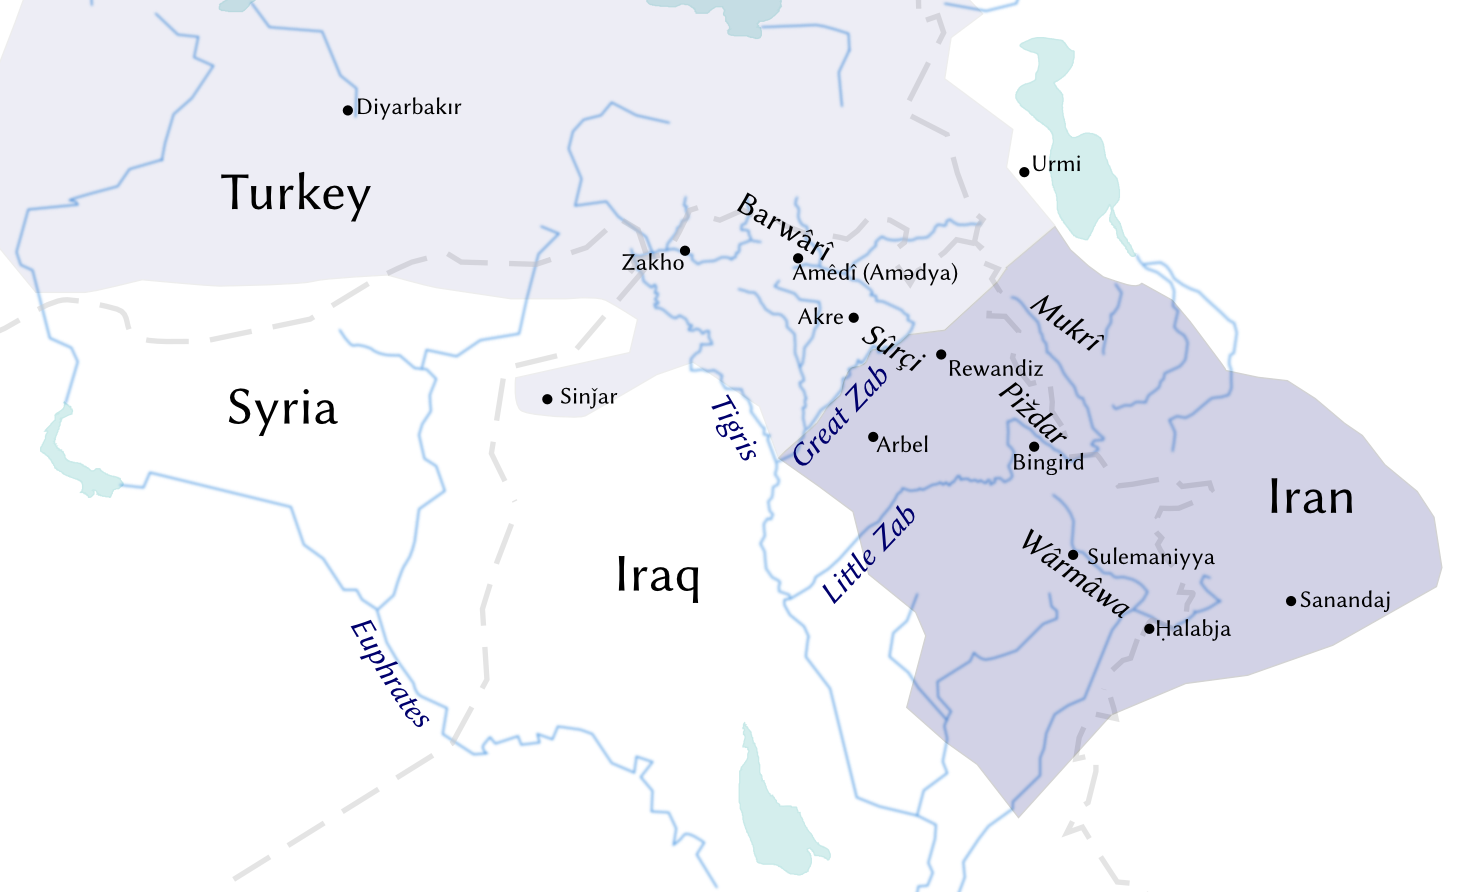
\includegraphics[width=\textwidth]{figures/Kurdishmap.png}
  \caption{Map of surveyed Kurdish dialects and localities. Light grey = Kurmanji dialects; dark grey = Sorani dialects.} \par \label{fg:map_kurdish} 
\end{figure}
  



The chapter is organised as follows: In \sref{ss:Kur_Poss} I treat the possessive pronominal enclitics, present only in \Sor dialects.  The most prominent AC markers in Kurdish are the various \ez* morphemes.  \Sref{ss:three_Ez} gives an overview of the  different forms found in standard Kurmanji and Sorani and motivates the differentiation of three distinct types of \ez* morphemes, discussed in the following sections. \Sref{ss:Kurdish_cst} discusses the Construct \ez* Construction, which can be seen as the Kurdish equivalent of the \ili{NENA} Neo-CSC. The marking of \secns by the \obl* case, present in Kurmanji dialects, is also discussed there.
\Sref{ss:lnk_ez} discusses the Linker \ez* Construction, which can be seen as the Kurdish equivalent of the \ili{NENA} ALC. 
\Sref{ss:Comp_Ez} discusses the usage of the Compounding \ez*, especially productive in \Sor. 
Clausal \secns appear regularly in one of the \ez* constructions, yet they can also appear in some alternative constructions, which are discussed in \sref{ss:Sor_alt_clause}.
The usage of the \isi{juxtaposition} construction, as well as the rare {inverse juxtaposition}\isi{inverse juxtaposition construction}, is presented in \sref{ss:Kur_Juxt}.
Finally, \sref{ss:Kurd_conclusions} concludes this chapter with some general remarks and comparative prospects. 

\largerpage
\section{Possessive pronominal enclitics (X-y.\poss)} \label{ss:Kurd_poss}
\label{ss:Kur_Poss}

Sorani (but not Kurmanji) has a series of unstressed possessive pronominal morphemes. \citet[15]{ThackstonSorani} qualifies them as enclitics, while \citet[76]{MacKenzie} treats them as suffixes. As these elements show promiscuous attachment, attaching indifferently to verbs (as objects; see \cite[37]{ThackstonSorani}), to nouns, and to prepositions, I prefer to analyse them as clitics (see \sref{ss:clitics_affixes}).\footnote{A thorough analysis of their status would require an investigation of their behaviour with verbal hosts, which is beyond the scope of this work. See, in this respect, \citet{SamvelianClitics}, who examines their attachment to verbs and prepositions and concludes, in a final account, that these elements are rather affixes.} 

The pronominal enclitics normally follow the definite or \isi{indefinite suffix}, with the expected meaning: 

\arabex[\Sor]{Noun}{Pronoun}{946}
{كوڕەكەم}
{kuř-eké \cb{}m}
{son-\defi{} \cb\poss.1\sg}
{my son}
{\citep[16]{ThackstonSorani}}

\arabex[\Sor]{Noun}{Pronoun}{834}
{كوڕێكم}
{kúř-êk \cb{}im}
{son-\indef{} \cb\poss.1\sg}
{a son of mine}
{\citep[16]{ThackstonSorani}}

When the noun is left unqualified, this typically yields  a figurative or generic meaning:

\arabex[\Sor]{Noun}{Pronoun}{832}
{كوڕم}
{kúř \cb{}im}
{son \cb\poss.1\sg}
{sonny (form of address for a young boy)}
{\citep[16]{ThackstonSorani}}

The possessive enclitics can appear after compound nominals consisting of a Noun+Adj. combination mediated by the compounding \ez* (see \sref{ss:Comp_Ez}).

\arabex[\Sor]{Compound Noun}{Pronoun}{836}
{كوڕە كۆرپەكەم}
{[kuř-e- korpe]-ké \cb{}m}
{son-\ez{}- newborn-\defi{}  \cb\poss.1\sg}
{my infant son}
{\citep[53]{ThackstonSorani}}

The same \isi{clitic} placement is found when the compounding \ez* is missing due to phonological conditions.  The following \War example can be compared to the \ili{NENA} \JSul \example{1104}:

\acex[\War]
{Compound Noun}{Pronoun}{911}
{[bira-gewr]-ek \cb{}em}
{brother-big-\defi{}  \cb\poss.1\sg{}}
{my elder brother}
{MacKenzie}{81 {[204]}}
 
Finally, the possessive enclitics can follow the focus \isi{enclitic} \foreign{-(î)ş}{also}.

\arabex[\Sor]{Noun}{Pronoun}{1945}
{پارەكەشیان}
{par-eké \cb{}ş \cb{}yan}
{money-\defi{} \cb{}also \cb\poss.3\pl}
{their money too}
{\citep[16]{ThackstonSorani}}

\arabex[\Sor]{Noun}{Pronoun}{835}
{رەفیقەكانیشم}
{refîq-ek-an \cb{}îş \cb{}im}
{friend-\defi-\pl \cb{}also \cb{}\poss.1\sg}
{even my friends}
{\citep[17]{ThackstonSorani}}


Note that in Kurmanji, the lack of possessive pronominal enclitics entails the use of full pronouns which are marked by the \isi{oblique case} (see \example{887}).

\section{The three Ezafe morphemes in Kurdish} \label{ss:three_Ez}

In \sref{ss:ezafe_dispute} I presented briefly the \Per \ez* and the dispute regarding its morphemic status (suffix or \isi{clitic}) and its syntactic attachment (with the \prim or the \secn). Since the \Per \ez* attaches phonologically to the \prim, I concluded, with Samvelian (\citeyear*{SamvelianEzafe, SamvelianHead}),
that the simplest account of the \Per \ez* is to view it as a \isi{phrasal affix} attaching morphologically and syntactically to its \prim, marking the latter as being in \cst*, i.e.\ wanting a complement. 

The situation in Kurdish dialects is somewhat more complex. First, in \Kur, the \ez* morpheme inflects for gender, number, and \isi{definiteness}. More importantly, there are  three distinct types of \ez* markers, differing in their phonological attachment:

\begin{description}

\item[Construct \ez*] Devoid of stress, attaching phonologically to the \prim (-\ez).

\item[Linker \ez*] Can carry stress, and can appear without an immediate \prim (\lnk.\ez).  

\item[Compounding \ez*] Devoid of stress, forming part of a nominal compound \linebreak (-\ez-).

\end{description}

 The various forms of the \ez* in standard Kurmanji and Sorani   are shown in \vref{tb:Ezafe_forms}.

\begin{table}[h!]
\centering
\begin{tabular}{llccc c}
\toprule
			&	& \multicolumn{3}{c}{Kurmanji} & Sorani \\

	&		& \masc 		& \fem 			& \pl		 &		\\
\midrule
\multirow{2}{*}{Construct} & \defi	& \transc{-ê}	& \transc{-a}	& \multirow{2}{*}{\transc{-ên}\footnotemark} & \multirow{2}{*}{\transc{-î}} \\
& \indef& \transc{-î}   & \transc{-e}	&	& \\

Linker & 	& \transc{yê}	& \transc{ya}	& \transc{yên} & \transc{hî} \\

Compounding	&	& \multicolumn{3}{c}{\transc{-e-}}	& \transc{-e-} \\
\bottomrule
\end{tabular}
\caption{The \ez* forms in Standard Kurmanji and Sorani} \label{tb:Ezafe_forms}
\end{table}

\footnotetext{In the Kurmanji dialects overlapping with \ili{NENA}, the regular marking of the plural \ez* is in fact \transc{-êd} or \transc{-êt} \citep[162]{OpenginHaig2014regional}.}

Leaving aside for the moment the compounding \ez*, I note that the (definite) construct \ez* and the Linker \ez* share the same form, except for a weak consonantal onset (\Kur: \phonemic{y-}; \Sor: \phonemic{h-}) marking the latter. In fact, in dialectal data this onset is absent at times. Thus, a natural assumption is to conflate the two sets, arguing these are prosodic variants of each other, one being an \isi{enclitic} and the other (possibly) a \isi{proclitic}. This is the approach taken by \citet[77]{HaigAlignment} and elaborated upon in \citet{HaigLinker}. Yet  as \citet{SamvelianHead} argues (for \Kur), there are distributional reasons for distinguishing the two series: The construct \ez* is in \isi{complementary distribution} with the \isi{oblique case} marking of nouns (present only in \Kur), and thus cannot attach to oblique nouns, while the \lnk* \ez*  is indifferent to the constitution of the \prim.

\acex[\Kur]
{Noun Phrase}{Adjective}{1949}
{[mal-a van jin-an] *-a / ya biçuk}
{house-\ez.\fem{} \dem.\near.\obl.\pl{} woman-\obl.\pl{} *-\ez.\defi.\fem{} / \lnk.\ez.\fem{} small}
{these women’s small house}
{SamvelianHead}{357, examples (47)--(48)}

\largerpage
Since the construct \ez* is in opposition to the \obl* case suffix, \citet[358]{SamvelianHead} analyses it as a suffix (or rather as a \isi{phrasal suffix}), similar to the \Per \ez*, while the \lnk* \ez* is analysed by her as an independent syntactic particle. A similar conclusion is reached by \citet[53]{SchroederAttribution}.
Recall that I used a similar approach to tease apart the \ili{NENA} \cst* suffix \ed and the \isi{proclitic} \lnk* \d (see \sref{ss:d_vs_ed}). 

\citet[79]{Haig2004} objects to this type of analysis (and in particular  to \cite{SchroederAttribution} noting that the \isi{complementary distribution} of the (construct) \ez* and the \isi{oblique case} is not restricted to cases where the \isi{oblique case} is realized by a suffix, but also in the relatively few nouns where the \isi{oblique case} is realized by an internal stem mutation. Thus, one finds \foreigngloss{cem şivan-ê me}{to shepherd-\ez 1\pl.\obl} meaning \transl{to our shepherd} and not \foreigngloss{*cem şivên-ê me}{to shepherd.\obl-\ez 1\pl.\obl}. While I concur with Haig that this demonstrates that the \isi{complementary distribution} of the two markers is not due to \enquote{a low-level constraint on suffix-stacking}, I disagree with his view that the \ez* is not inflectional in nature. In fact, this evidence strengthen the position that the construct \ez* is an inflectional element, as it shows the the \isi{oblique case} marking and the construct \ez* are part of the same abstract paradigm in the Kurmanji linguistic system (a case-cum-state paradigm, as it is), irrespective of the actual realisation of the members of the paradigm. Since the case marking (suffixal or by stem mutation) is clearly inflectional, the same must hold for the \ez*.  

In this study I adhere to Samvelian's analysis, and I shall treat the different types of  \ez* in different sections below. It should be noted, though, that this analysis is especially suitable for \Kur. In \Sor there are no inflectional case endings, and thus the above argument is not applicable.\footnote{In \Sor, on the other hand, nouns can be inflected by the possessive enclitics, discussed in \sref{ss:Kurd_poss}. It would be interesting to see if the construct \ez* is compatible with these enclitics, but unfortunately I have not found data regarding this question. \label{ft:sor_poss_infl}} Yet, as the \Sor construct \ez* appears only after nominal elements (the linker \ez* occurring only without an immediate \prim), it can be seen as a nominal suffix, and therefore I treat  it for simplicity's sake on a par with the \Kur construct \ez*.
 
 
\section{The construct Ezafe construction (X.\textsc{cst} Y)} \label{ss:Kurdish_cst}
\subsection{Introduction}
As explained above, all Kurdish dialects make use of the construct \ez*, a suffix attaching to the \prim phrase, marking it as \cst*. The different varieties of Kurdish differ as to the number of inflectional forms the \ez* exhibits, reflecting various number and gender distinctions. Generally speaking, the number of forms increases as one travels from the south-eastern extremity of Kurdish speaking areas to the north-western extremity. In this perspective, it is useful to take into account also dialects of languages close to Kurdish, such as \ili{Gorani} in the south-east and \ili{Zazaki} in the north-west.\footnote{See \vref{ft:gorani_zazaki} for a discussion of various classifications of these languages.}

In the southern part of my survey of Kurdish dialects, namely in the Sorani dialects, the construct \ez* has a fixed form \transc{-î}\~\transc{-i}\~\transc{-y}.\footnote{\citeauthor{ThackstonSorani} transcribes the \ez* as a lax \transc{i}, separated from its host. Other authors, however, as well as the standard Sorani \ili{Arabic} orthography, treat the \ez* as a tense \transc{î} (in \ili{Arabic} script: \textarabic{ی}), attached to its host. After vowels it is realised as the glide \phonemic{y}. In line with my analysis of the \ez* as a suffix, I transcribe it attached to its host, but I keep the formal variation intact.} Note that the usage of an uninflected \ez* is found also in the \Gawr \ili{Gorani} dialect, spoken in the southern extremity of the Kurdish speaking zone, near the city of Kerend \citep[16]{MahmoudveysiGawraju}; this \ez* has the form \transc{-e}\~\transc{-y}, akin to the uninflected \Per \ez* \transc{-(y)e}.

\arabex[\Sor]{Noun}{Noun}{821}
{كتاویەكانی قوتابخانەیەك}
{ktawî-ek-an-i qutabkhane-yêk}
{student-\defi-\pl-\ez{} school-\indef}
{the students of a school}
{\citep[10]{ThackstonSorani}}

\acex[\KSul]{Noun}{Noun}{897}
{ser-î binîâdem}
{head-\ez{} man}
{men's heads}
{MacKenzie}{63 {[49]}}

As \example{821} shows, the \prim and \secn can be independently marked as definite or indefinite. If they are left unmarked, as in \example{897}, the AC may be interpreted generically.

The same construction can be used with a full pronominal \secn, as an alternative to the usage of the possessive enclitics (see \sref{ss:Kur_Poss}), for \enquote{special emphasis} \citep[179]{AbdullaMcCarus}.

\acex[\KSul]{Noun}{Pronoun}{945}
{nàv-i mín}
{name-\ez{} 1\sg}
{\textit{my} name}
{AbdullaMcCarus}{179}


As one travels northwards, roughly to the \emph{Inter-Zab}\il{Inter-Zab dialects} region (between the Little Zab and the Great Zab rivers), more variation appears. In some Sorani dialects (namely, \Muk and \Rdz) the \ez* may appear as \transc{-(y)e} following a vowel \citep[62]{MacKenzie}. 

\acex[\Rdz]{Noun}{Pronoun}{882}
{kursî-(y)e min}
	{seat-\ez{} 1\sg}
{my seat}
{MacKenzie}{62 {[484]}}

 This is purely a phonological variant of the \ez*. More interesting  is that some north-eastern Sorani dialects (\Bin, \Piz and \Muk) exhibit an optional \ez* form, \transc{-ê}, reserved for \fem* \sg* nouns \citep[61]{MacKenzie}. This is shown by the following example:
 
 \acex[\Muk]{Noun}{Proper Noun}{877}
 {xuşk-ê Mîr Zêndîn}
 {sister-\ez.\fem{} M. Z.}
 {Mir Zendin's sister}
 {MacKenzie}{61 {[30]}}
 
  In the same dialects, whenever the \prim has plural sense but no formal marking of this (as an unmarked noun can be interpreted singularly or plurally), an extra particle \transc{de} may follow the \ez*.\footnote{It is a curious fact that this \pl* \ez* marker has a  similar form to the Aramaic \lnk* \d. Yet, as the Aramaic \lnk* is not related in any way to marking of plurality, this is very likely a pure coincidence.}
  
  \acex[\Bin]{Noun}{Noun}{883}
  {pyaw-î de paşe}
  {man-\ez{} \pl{} king}
  {the king's men}
  {MacKenzie}{62 {[319]}}
  
  The same marker is used whenever the \prim consists of a conjunction of two singular nouns. In such cases, the \ez* is attached phrase-finally. 
  
   \acex[\Bin]{Conjoined nouns}{Pronoun}{887}
   {[dak û bab]-î de to}
   {mother and father-\ez{} \pl{} 2\sg}
   {thy mother and father}
   {MacKenzie}{62 {[349]}}
 
  Among the Kurmanji dialects, a distinction between the two genders is obligatory, as is shown in \vref{tb:Ezafe_forms}. Most dialects also have a separate \pl* \ez*, though sometimes it is assimilated with the \masc*  \sg* form. The usage of the \pl* form as well as the \fem* form is shown in the following example, which shows also the possibility to embed the \ez* construction:
  
  \acex[\Kur]{Noun}{Noun Phrase}{711}
  {kitêb-ên [keç-a mirov]}
  {book-\ez.\defi.\pl{} girl-\ez.\fem{} man}
	  {the man's daughter's books}
  {ThackstonKurmanji}{13}
  
  In some older literary texts, one finds the same plural particle as in the Sorani dialects mentioned above (see \examples{883}{887}). Such is the case, for instance, in the poetry of the Kurdish poet Malaye Jaziri of Bohtan (1570-1640)\footnote{These years are given by \citet[176]{IzadyKurds}, who writes the poet's name as \textit{Mullâ-i Jaziri}.}:
  
  \arabex[\Kur]{Noun}{Adjective}{891}
  {چشمین دِ سِيَه}
  {çeşm-ên di siyeh}
  {eye-\ez.\defi.\pl{} \pl{} black}
  {black eyes}
  {(Malaye Jaziri, \textit{Diwân}, ed.\ \cite[217]{Hartmann}; \cite[159, fn.\ 2]{MacKenzie})}
  
The \Kur \ez*, just like the \Sor \ez* shown in \example{887}, attaches phrase-finally to the \prim, and has scope over the whole \prim phrase. According to the description of \citet{BedirKhan}, the inflectional features carried by the \Kur \ez* suffix are, however, only dependent on the noun to which it directly attaches (this is also the case in \example{752}, cited from \citeauthor{ThackstonKurmanji}):\footnote{One reviewer noted that this is not a strict rule but subject to dialectal variation, bringing the following example from the Zakho dialect: \foreigngloss{kič u kur-ēt min}{daughter and son-\ez.\pl{} 1\sg.\obl} meaning \transl{my daughter and son}. Note that the plural \ez* is used due to the plurality of the NP but attaches to a singular noun.} 



 \acex[\Kur]{Conjoined nouns}{Pronoun}{950}
 {[dê û bav]-ê min}
 {mother and father-\ez.\defi.\masc{} 1\sg.\obl}
 {my mother and father}
 {BedirKhan}{2}
 
 \acex[\Kur]{Conjoined nouns}{Pronoun}{951}
  {[ker, hesp û mehîn]-a min}
  {donkey, horse and mare-\ez.\defi.\fem{} 1\sg.\obl{}}
  {my donkey, horse and mare}
  {BedirKhan}{2}
 
 
 This behaviour indicates that the \Kur \ez* should be analysed as a \isi{phrasal suffix}: while morphologically it is tied to the nominal inflectional system and thus shows inflectional features of the noun it attaches to, syntactically it marks the entire NP as being in \cst* and  has thus wide syntactic scope (see \sref{ss:clitics_affixes} and in particular \vref{tb:continuum}).
 
Likewise, if the last noun of the \prim has a plural sense by itself, it will receive the \pl* \ez* suffix. In such cases the \pl* sense may be inferred pragmatically also for the other conjunct nouns of the \prim, as in the following example:\footnote{Note that a \Kur noun without \ez* or \obl* case marking is unmarked for number, and may be interpreted either as \pl* or as \sg* according to the context.}
  
\acex[\Kur]{Conjoined nouns}{Noun}{724}
{[şexsiyet û rewşenbîr]-ên kurd-an}
{personality(\fem) and intellectual-\ez.\defi.\pl{} Kurdish-\obl.\pl{}}
{personalities and intellectuals of the Kurds}
{ThackstonKurmanji}{15}


 
  \citeauthor{BedirKhan}  notes that this pattern  only arises with the conjunction \foreign{û}{and}. When the \prim NP consists of nouns joined using the disjunctive conjunction \foreign{(y)an}{or}, each element must belong to a separate AC.   
 
 \acex[\Kur]{Disjoined Nouns}{Pronoun}{952}
 {hesp-ê min an mehîn-a min}
 {horse-\ez.\defi.\masc{} 1\sg.\obl{} or mare-\ez.\defi.\fem{} 1\sg.\obl}
 {my horse or my mare}
 {BedirKhan}{2}
  
  
  The \Kur \ez* inflects also according to the \isi{definiteness} of the noun.  Yet, in contrast to its number and gender inflection, the (in)\isi{definiteness} feature is  not carried by the \ez* suffix, but rather it co-varies  with the presence of a singular \isi{indefinite suffix} \transc{-êk} \citep[158-160]{MacKenzie} or a plural \isi{indefinite suffix} \transc{-in} \citep[78]{BedirKhanLescot}. 
  
  \acex[\Kur]{Noun}{Noun}{708}
  {hejmár-ek-e kovár-ê}
  {issue(\fem)-\indef-\ez.\indef.\fem{} journal-\obl.\fem{}}
  {an issue of that journal}
  {ThackstonKurmanji}{12}\antipar
  
  
   \newpage
  \acex[\Kur]{Noun}{Noun}{949}
  {mehîn-in-e keçk-ê}
  {mare-\pl.\indef-\ez.\indef.\pl{} girl-\obl.\fem}
  {some mares of the girl}
  {BedirKhanLescot}{306}\antipar
    
  
  Since these allo-forms depend on the explicit presence of an \isi{indefinite suffix}, \citet[355-357]{SamvelianHead} rejects the notion of the \concept{indefinite ezafe}, analysing these forms instead as being conditioned by their post-affixal position. She shows that an indefinite \pl* noun not marked by the suffix \transc{-in} takes the normal form of the \ez*  \transc{-ên}:
  
  \acex[\Diar]
  {Noun}{Adjective}{1950}
  {pênc kur-ên ganc}
  {five boy-\ez.\pl{} young}
  {five young boys}
  {SamvelianHead}{356, example (45)}
  
  This pattern, however, could equally well be analysed as a neutralisation of the \isi{definiteness} feature of the \pl* \ez* (as presented in \vref{tb:Ezafe_forms}). Such a neutralisation may be motivated by the fact that the explicit marking of \pl* indefinite nouns by means of the   suffix \transc{-in} is quite rare (judging by the sources consulted), and that the indefinite \pl* \ez* \transc{-e} is  identical in form to the indefinite \fem* form, as is shown in \examples{708}{949}.
  
  \citet[356]{SamvelianHead} substantiates further her claim by citing   \citet[158]{MacKenzie}, who mentions that in \Sur dialect, the indefinite form (termed by him \concept{secondary ezafe}), follows \enquote{apparently} also the \isi{definite suffix} \transc{-eke}:
  
  \acex[\Sur]
  {Noun}{Adjective}{1951}
  {mirow-eke-y xwarê}
  {man-\defi-\ez.\masc{} lower}
  {the lower man}
  {MacKenzie}{160 {[517]}}
   
  Yet  most \Kur dialects lack the \isi{definite suffix} \transc{-eke}, which is more typical of \Sor dialects. Thus, leaving aside such exceptional examples (whose status seems to be questioned by \citeauthor{MacKenzie} himself), it seems justifiable to regard the \sg* \ez* forms \transc{-î} (\masc) and \transc{-e} (\fem) as allomorphic forms signalling indefiniteness of the \prim noun.\footnote{Note, however, that \transc{-î} is also used in some contexts where no indefiniteness is implied, such as with \isi{adverbial} \prims (see \sref{ss:cst_ez_adv_prim}).}
  
  


The same cline of explicitness can also be found regarding the marking of the \secn by  \isi{oblique case}. This is treated in \sref{ss:Kurd_obl}.




\subsection{Oblique marking of \secns} \label{ss:Kurd_obl}


\Kur exhibits a bipartite case system, opposing the unmarked direct case with a marked \isi{oblique case}, visible on nouns and pronouns. On nouns, the \isi{oblique case} is normally marked by suffixes, which express moreover the gender and number features of the host noun. These suffixes are shown in \vref{tb:Obl_forms}.

\begin{table}[h!]
\centering
\begin{tabular}{l ccc}
\toprule
			&	\masc & \fem & \pl \\
\midrule
Direct		& \multicolumn{3}{c}{\zero} \\
Oblique		& \zero\ / \transc{-î}	& \transc{-(y)ê}	& \transc{-(y)an} \\
\bottomrule
\end{tabular}
\caption{Kurmanji case endings} \label{tb:Obl_forms}
\end{table}

A particularity of the \masc* \sg* oblique suffix is that it appears only if the host noun is qualified by a determiner.\footnote{This is the rule in Standard Kurmanji. Yet in the Kurmanji dialects overlapping with the \ili{NENA} speaking zone, there is a consistent suffix-marking of the oblique. See the discussion of \citet[162]{OpenginHaig2014regional} and \citet{HaigOpengin2017structure} regarding the \enquote{Southeastern} Kurmanji dialect group.} 
Yet a few masculine nouns show the \isi{oblique case} by internal mutation, replacing an ultimate \phonemic{a} vowel by an \phonemic{ê} vowel \parencites[9]{ThackstonKurmanji}[73]{Haig2004}. For example, \foreign{bajar}{city} is \transc{bajêr} in the \isi{oblique case} (see \example{955}).

The \isi{oblique case} marks the dependents of both the \isi{attributive relation} and the \isi{completive relation} (see \sref{ss:threeRel}). It subsumes thus both the \isi{genitive case} and the accusative case (and in the \Kur context, also the ergative case). Note, moreover, that similarly to the \ez* the oblique suffixes can have phrasal scope, appearing on the final noun of conjoined nouns, and only optionally on the preceding nouns.\footnote{In this respect it is also somewhat different to the \ez*, as the \ez* can only appear on the last conjoined noun, since it must be followed immediately by the \secn.} This is demonstrated by the following example, in which the \obl* case takes the accusative role.

\acex[\Kur]
{Verb}{Conjoined Nouns (objects)}{Sam_Obl}
{[jin-\opt{ê} u kur-î] di-bîn-im}
{woman-\opt{\obl.\fem} and boy-\obl.\masc{} \ind-see-1\sg}
{I see the woman and the boy}
{SamvelianHead}{354, example (41)}\antipar\antipar

\newpage 
In this study, I am interested mainly in the \gen* function of the \obl* case, namely the marking of AC \secns. This is shown in the following example (as for the oblique demonstrative, see \vref{tb:kur_dem}):

\acex[\Kur]{Noun}{Noun}{706}
{miróv-ek-î  [w-î weláṭ-î]}
{man-\indef-\ez.\indef.\masc{} \dem.\far-\obl.\masc{} country-\obl.\masc}
{a man of that country}
{ThackstonKurmanji}{12}

For examples of \fem* and \pl* oblique endings, see \examples{724}{708}.

It is important to note that the \ez* suffix and the \obl* marking (suffixal or by stem mutation) are morphologically in \isi{complementary distribution}, although notionally they mark independent features, the \ez* being related to the state category.\footnote{\textit{Pace} \citet[7]{ThackstonKurmanji} who speaks of construct \enquote{case}. In the \ili{Zazaki} language, related to Kurmanji, a noun can be marked both for \isi{oblique case} and the \isi{construct state} by means of a specially inflected \ez* \parencites[43]{Todd}[and see further][]{LarsonYamakido}{SamvelianHead}{PlankSuffixaufnahme2012}. See also the discussion at the end of \sref{ss:three_Ez}.} Thus, a \secn noun itself acting as \prim is only marked by the \ez*. An \obl* suffix, if present at all, can only be marked in such cases at the end of the \secn phrase:

\acex[\Kur]
{Circumposition}{Noun Phrase}{713}
{di [gund-ên kurd-ên Kurdistan-a Tirkiye-yê] de}
{in village-\ez.\pl{} Kurd-\ez.\pl{} Kurdistan-\ez.\fem{} Turkey-\obl.\fem{} in}
{in the villages of the Kurds of Turkey's Kurdistan}
{ThackstonKurmanji}{13}

Kurmanji dialects also have  a series of full oblique pronouns, which can be used as \secns. These are the functional equivalents of the Sorani possessive pronominal enclitics, described in \sref{ss:Kurd_poss}. For example, the direct pronoun \foreign{ez}{I} has the oblique form \transc{min} (see its occurrence also in \examples{950}{951}):

\acex[\Kur]{Noun}{Pronoun}{743}
{kitêb-a min}
{book-\ez.\defi.\fem{} 1\sg.\obl}
{my book}
{ThackstonKurmanji}{18}

\newpage 
In contrast to nouns, an oblique pronoun can further be marked by the \ez* suffix:\footnote{Yet  this may in fact be an instance of the linker \ez* discussed in \sref{ss:lnk_ez} phonologically encliticized to the \prim, as it does not necessarily show the inflectional features of its host pronoun, as would be expected from the construct \ez*. Thus, in the following example, the \ez* suffix \transc{-a} shows agreement with the \prim \foreign{mal}{house} rather than with the pronoun \transc{min} (given that the speaker is a man):

\acexfn[\Kur]
{Pronoun}{Noun}{1954}
{mal-a [bira-yê min]-a biçuk}
{house.\ez.\fem{} brother-\ez.\masc{} 1.\sg.\obl-\ez.\fem{} small}
{my brother's small house}
{SamvelianHead}{354, example (40)}
 
See \example{768} for a clear case of the \lnk* \ez* following \transc{min}.
 }

\acex[\Kur]
{Pronoun}{Noun}{1953}
{min-ê bêçâra bibîna}
{1.\sg.\obl-\ez.\masc{} poor look.\imp}
{Look at me, poor thing}
{SamvelianHead}{353, example (39)}

In contrast to Kurmanji, the south-eastern Sorani dialects (and notably the dialect of Sulemaniyya, which is the basis for standard Sorani) have no case system at all. The Sorani dialects to the north, however, show an oblique suffix for singular \secns:\footnote{The \pl* is marked by a case-neutral suffix \transc{-ân} \citep[58]{MacKenzie}.}

\acex[\Bin]{Noun}{Noun}{898}
{lep-î dest-î}
{palm-\ez{} hand-\obl.\masc{}}
{palm of the hand}
{MacKenzie}{59}

\acex[\Bin]{Noun}{Noun}{899}
{zîn-î maîn-ê}
{saddle-\ez{} mare-\obl.\fem{}}
{saddle of the mare}
{MacKenzie}{59}

\newpage 
\subsection{Adjectival \secns}


The \ez* construction is used also with adjectival \secns. In \Kur, adjectives differ from nouns by the fact that they never inflect and thus do not take an \obl* suffix \citep[163]{MacKenzie}.\footnote{Note, however, that the denominal adjective derivational suffix \transc{-î} is conspicuously similar to the \masc* \sg* oblique ending, making an historical connection between the two possible. This recalls the situation in the \ili{Semitic} domain, where  a formal similarity can be observed between the \Arab adjectival ending \transc{-iyy} and the \gen* case \transc{-i}. The usage of the oblique suffixes as derivational suffixes is much clearer in the case of the \Kur \isi{ordinals}; see \ref{ss:kurd_ez_ord}.}


\acex[\Kur]{Noun}{Adjective}{715}
{mirov-ek-î mezin}
{man-\indef-\ez.\indef.\masc{} big}
{a big man}
{ThackstonKurmanji}{14}

\acex[\KSul]{Noun}{Adjective}{893}
{tûtik-êk-î piçkołe}
{dog-\indef-\ez{} small}
{a little dog}
{MacKenzie}{63 {[69]}}


As the above examples show, the \prim can be determined by the \isi{indefinite suffix} in both \Kur and \Sor. In Kurmanji dialects, a definite sense is obtained by using the definite \ez*:

\acex[\Kur]{Noun}{Adjective}{714}
{mirov-ê mezin}
{man-\ez.\defi.\masc{} big}
{the big man}
{ThackstonKurmanji}{14}

\largerpage
In Sorani, however, a \prim noun followed by an adjective is not normally combined with the \isi{definite suffix} \transc{-eke}. Instead, whenever a definite \prim is needed, the compounding \ez* is used (see \sref{ss:Comp_Ez}). It seems, however, that the construct \ez* construction is compatible with a definite \prim, if the adjective has a descriptive, rather than restrictive, sense \citep[see][12, fn.~1]{ThackstonSorani}. 

\arabex[\Sor]
{Noun}{Adjective}{831}
{دەرسەكانی سەخت}
{ders-ek-an-i sext}
{lesson-\defi-\pl-\ez{} hard}
{the lessons, which are hard}
{\citep[12]{ThackstonSorani}}\antipar 

\newpage 

Whenever a \prim is modified by more than one adjective, several alternative patterns are available. The adjectives may be conjoined to form one \secn phrase:

\acex[\KSul]{Noun}{Conjoined Adjectives}{903}
{minał-êk-î [pîs û poxił]}
{child-\indef-\ez{} dirty and filthy}
{a filthy, dirty child}
{MacKenzie}{63}

\acex[\Kur]{Noun}{Conjoined Adjectives}{947}
{keç-ên [por-zer û çav-şîn û kesk]}
{woman-\ez.\pl{} hair-yellow and eye-blue and green}
{blonde and blue- and green- eyed women}
{ThackstonKurmanji}{98}

Another possibility is to chain the subsequent adjectives by \ez* suffixes, as the following Sorani examples show. In such cases one might expect the two adjectives to have  different scopes (the first qualifying the \prim noun only, while the second qualifies the N+Adj. combination), yet this is not apparent from the translations:

\arabex[\Sor]{Noun}{Adjectives}{852}
{شارێكی گەورەی تازە}
{[shar-êk-î gewre]-y taze}
{city-\indef-\ez{} big-\ez{} modern}
{a big modern city (\textit{une grande ville moderne})}
{\citep[60]{BlauSorani}}

\acex[\KSul]{Noun}{Adjectives}{904}
{[kiç-êk-î jwan]-î çwar-de \cb{}sał}
{girl-\indef-\ez{} pretty-\ez{} four-teen \cb{}year}
{a beautiful, fourteen-year-old girl}
{MacKenzie}{63}

\largerpage
This latter possibility seems to be unavailable for Kurmanji dialects, which instead make use of the \lnk* \ez* construction  in such cases (see \sref{ss:lnk_ez}).\footnote{See however the rare usage of the \Kur \lnk* \ez* \transc{î} in \examples{742}{955}, which, notwithstanding the difference in analysis, is very similar formally to the construct \ez* in  the  above cited \Sor examples.}  
This is correlated with the fact that the Kurmanji \ez* is a nominal inflectional suffix, incompatible with adjectives, which never inflect. The \Sor \ez*, on the other hand, does not \emph{prima facie} form part of an inflectional system, and in this respect shows \isi{clitic} behaviour (but see \vref{ft:sor_poss_infl}). 



\subsection{Adjectival \prims}

In Sorani, one finds that adjectives extended by nominal complements get the \ez* suffix: 

\acex[\Muk]{Adjective}{Noun}{914}
{xerîk-î bezm-î (de-bû-n)}
{busy-\ez{} feasting-\obl(?) \ind-be-\pl}
{(They would be) engaged in feasting.}
{MacKenzie}{65 {[3\textsuperscript{25}]}}

\acex[\KSul]{Adjective}{Noun}{915}
{tûş-î em derd-e}
{afflicted-\ez{} \dem.\near{} trouble-\defi}
{afflicted by this trouble}
{MacKenzie}{65 {[67]}}

Note that \example{914} is very similar to the \ili{NENA} \JSan \example{98}. 

In \Kur, such examples are not expected to be found, as adjectives are normally not marked by the construct \ez* (see discussion at the end of the previous section). Yet  \citet[343]{SamvelianHead} affirms the existence of this construction:

\acex[\Kur]
{Adjective}{Noun}{1946}
{Azâd âşiq-ê Narmîn-ê ya}
{A. in\_love-\ez.\masc{} N.-\obl.\fem{} \cop.3\masc}
{Azad is in love with Narmin.}
{SamvelianHead}{343, example (15)}

Note, however, that \citet[197]{ThackstonKurmanji} lists this construction only in combination with the verb \transl{to be} (\transc{ʿaşiq-e ... bûn}), rendering it possibly a fixed collocation. 

\subsection{Ordinal \secns} \label{ss:kurd_ez_ord}
\largerpage[1.5]
Ordinals follow the \ez* as regular \secns. In standard \Kur they are derived from the cardinal numerals by a fixed \obl* \pl* suffix \transc{-yan}, except for the \isi{numeral} \transl{first}, which has a special form \transc{ewel(î)} in which one can recognize the \masc* \sg* \obl* ending \transc{-î}. Alternatively, \isi{ordinals} (including \transl{first}) may be derived by taking the suffix \transc{-ê(m(în))} of \Per origin \citep[25]{ThackstonKurmanji}.\footnote{According to \citet[170, \S 274.(a)]{MacKenzie}, the \Kur dialects form \isi{ordinals} by the  suffix \transc{-ê} (see \example{808}), which he relates to the identically formed superlative suffix \citep[164, \S 268.(b)]{MacKenzie}. In this case, it is the equivalent of \Sor suffix \transc{-în}, serving as a superlative \citep[68, \S 190.(b)]{MacKenzie}; see \vref{ft:superlative_ordinals}.\label{ft:superlative_e}}

\acex[\Kur]{Noun}{Ordinal}{750}
{roj-a sisi-yan}
{day-\ez.\defi.\fem{} three-\obl.\pl}
{(on the) third day}
{ThackstonKurmanji}{25}

\acex[\Kur]
{Noun}{Ordinal}{1952}
{car-a yeḳ-em}
{time-\ez.\defi.\fem{} one-\ord}
{the first time}
{ThackstonKurmanji}{25}

 In Sorani, \isi{ordinals} are similarly derived from the cardinal numerals by means of the suffix \transc{-(h)em} \citep[72--73]{MacKenzie}.

\acex[\KSul]{Noun}{Ordinal}{924}
{řêga-y sê-hem}
{third-\ez{} three-\ord}
{the third road}
{MacKenzie}{72 {[47]}}

 Alternatively, \Sor uses a longer ordinal suffix \transc{-(h)emîn} (borrowed in  \ili{NENA} \JUrm  and \JSan; see \example{130} and \example{281}). Yet when  \isi{ordinals} are derived by the full suffix \transc{-emîn}, they are not used in the \ez* construction, but rather in the \isi{inverse \isi{juxtaposition} construction} (see \example{1915}).


\subsection{Adverbial \secns} \label{ss:cst_ez_adv_secn}

In Kurmanji, prepositional phrases can regularly occur as \secns following the construct \ez*:\footnote{The usage of \cst* marker followed by \PP s is known also in the Aramaic domain. For Syriac, see \examples{1116}{1151}; for \JZax, see \examples{378}{377}; \JUrm: \example{148}.}

\acex[\Sor]{Noun}{\PP}{722}
{rojname-yek-e [bi kurdî]}
{newspaper-\indef-\ez.\indef.\fem{} in Kurdish}
{a newspaper in Kurdish}
{ThackstonKurmanji}{14}

In Sorani, this construction is not mentioned in the sources consulted, except by  \citet[346]{SamvelianHead}, who lists it as a regular construction:

\acex[\Sor]
{Noun}{\PP}{1948}
{xânu-y [la sar şâx]}
{house-\ez{} at head mountain}
{the house on the mountain}
{SamvelianHead}{346, example (19)}



\subsection{Adverbial  \prims} \label{ss:cst_ez_adv_prim}

Some nominals and adverbs can be used as prepositions. 
In \Kur, they may be marked by a frozen uninflected \ez* \transc{-î} termed by \citet[200]{MacKenzie} the \concept{generic ezafe}. Note, moreover, that complements of prepositions in \Kur are regularly marked by the \obl* case. 



\acex[\Ak]{Adverbial Noun}{Noun}{784}
{nêzîk-î ḥakim-i}
{near-\ez{} judge-\obl.\masc}
{near the judge}
{MacKenzie}{161 {[602]}}


See also \example{752} for the usage of the circumposition \foreigngloss{ji ali-yê ... ve}{from side-\ez.\masc\ ... from} introducing a passive agent. 

In \Sor, an \isi{adverbial} noun is similarly sometimes marked by the \ez* (but see \example{1955}):

\acex[\KSul]
{Adverbial Noun}{Pronoun}{943}
{la dwâ-y min}
{at last-\ez{} 1\sg}
{after me}
{AbdullaMcCarus}{75}

\subsection{Verbal nouns as \prims} \label{ss:cst_ez_verbal}

Verbal nouns, be they infinitives or nouns participating in complex predication (CP nouns), can be complemented by an argument following the construct \ez*.\footnote{Compare this to the situation in Aramaic; \Syr \isi{participles}: \examples{1151}{1117}; \JZax infinitives: \sref{ss:JZax_inf_head}; \Qar infinitives: \sref{ss:Qar_CSC_inf} \JUrm \isi{participles}: \example{122}; \JSan CP noun: \example{49}.} Note that \Kur infinitives have feminine gender and are hence marked by \fem\ \ez* \citep[32]{ThackstonKurmanji}. 

\acex[\Kur]{Infinitive}{Pronoun (subject)}{768part}
{çûyîn-a min}
{go.\inf-\ez.\defi.\fem{} 1\sg.\obl{}}
{my going}
{}{(\cite[33]{ThackstonKurmanji}; see \example{768} for a fuller context)}

\arabex[\Sor]
{Infinitive}{Noun Phrase (object)}{828}
{بۆ توانینی ئەم دیاری جێگای میر گەورەیە}
{bo twanîn-i [em dyarî kirdin-i [cêga-i Mîr Gewre] \cb{}yé]}
{for be\_able.\inf{}-\ez{} \dem.\near{} clarification do.\inf{}-\ez{} position-ez{} M. G. \cb{}\defi  }
{in order to enable this clarification of Mir Gawra’s position}
{\citep[12]{ThackstonSorani}}




\acex[\KSul]{CP Noun}{Noun (object)}{913}
{swar-î řexş bû}
{horseman-\ez{} steed was}
{He mounted his steed.}
{MacKenzie}{65 {[66]}}

The argument occupying the \secn can also be an indirect object. Such is the case in the following example, in which the direct object \transc{vê kaġez-ê} is governed directly by the verb, while the indirect object is governed by a CP noun. 

\acex[\Ak]{CP Noun}{Noun (indirect object)}{788}
{vê kaġez-ê teslîm-î [filan wezîr-î] bi-k-e}
{\dem.\near.\obl{} letter-\obl.\fem{} giving-\ez{} such\_and\_such vizier-\obl.\masc{} \subj-do-2\sg}
{Give this letter to such and such a vizier!}
{}{(\cite[161]{MacKenzie}; \cite[274]{MacKenzieTexts} {[603]})}















\subsection{Clausal \secns and the use of the relativizer} \label{ss:cst_ez_clausal}

Relative clauses, or, in other words, clausal \secns, make use of the \ez* construction as well, with the addition that normally a special particle, a \isi{relativizer}, introduces the clause. Thus, the \ez* signals that the \prim is to be modified, while the \rel* marks the clause as a \secn.\footnote{In Sorani, \citeauthor{ThackstonSorani} distinguishes between the \ez* introducing a \isi{relative clause}, being a tense \transc{-î}, and the regular \ez*, being a lax \transc{i}. As we have seen, other authors transcribe the regular \ez* as a tense \transc{î} as well, rendering this distinction apparently artificial.} In Sorani, the \rel* is \transc{\textarabic{كە} ke} while in Kurmanji it is \transc{ḳu}.\footnote{\citet{HaigLinker} treats  \transc{ḳu} as a \isi{complementizer}, while \citet{ThackstonKurmanji} regards it as a relative pronoun. Since the current study deals here only with cases where \transc{ḳu} is followed by a \isi{relative clause}, I will treat it as a \isi{relativizer} (glossed \rel), without committing to its general status. Recall that the under-dot of \phonemic{ḳ} signals an unaspirated and/or pharyngealized consonant, a phonemic distinction that is normally not marked in standard \Kur orthography (\citeauthor[4]{ThackstonKurmanji} marks it with an underscore and describes it as an unaspirated stop accompanied by pharyngealization \phonetic[kˁ].} 

\arabex[\Sor]{Noun}{Clause}{837}
{سەری كوڕەكەی كە نوستبوو}
{ser-i [kuř-eké-î ke nustibû]}
{head-\ez{} boy-\defi-\ez{} \rel{} slept.3\masc}
{the head of the boy, who has fallen asleep}
{\citep[73]{ThackstonSorani}}

\arabex[\Sor]{Noun}{Clause}{872}
{ئەو كراسەی كە تۆ كـڕیوتە}
{ew kiras-e-y ke [to kiřî-w-t-e] (zor drêj \cb{}e)}
{\dem.\far{} dress-\defi-\ez{} \rel{} 2\sg{} bought-\prf-2\sg-\cop.3\sg{} very long \cb{}\cop.3\sg}
{The dress that you bought (is very long).}
{\citep[156]{BlauSorani}}

\acex[\Kur]{Noun}{Clause}{753}
{wî ziman-ê ḳu [li ber mirinê ye]}
{\dem.\far.\obl{} language-\ez.\defi.\masc{} \rel{} at fore die.\inf.\obl.\fem{} \cop.3\sg}
{this language, which is on the verge of dying}
{ThackstonKurmanji}{75}

\acex[\Kur]{Noun Phrase}{Clause}{752}
{[ew alfabe û rêziman]-a ḳu [ji ali-yê Celadet Bedir-Xan ve haṭiye danîn]}
{\dem.\far{} alphabet and grammar-\ez.\defi.\fem{} \rel{} from side-\ez.\masc{} C. B.-X. from \pass.\prf{} put\_down.\inf}
{the alphabet and grammar that were established by Djeladet Bedir Khan}
{ThackstonKurmanji}{75}\antipar\antipar 
\newpage 

The \rel* can be omitted, especially (but not exclusively) when the \prim refers to the object of the subordinated verb, according to  \textcites[73]{ThackstonSorani}[77]{ThackstonKurmanji}. \citet[157]{BlauSorani}, however, relates its omission to the definite marking of the \prim.


\arabex[\Sor]{Noun Phrase}{Clause}{843}
{ئەو دوو فرمێسكە گەورەیەی ئەیانەوێ  بكەونە خوارێ}
{[ew dû firmêsk-e- gewre-yé]-î [e-yan-ewê bi-kew-in-à xwarè]}
{\dem.\far{} two tear-\ez- big-\definite{}-\ez{} \ind-3\pl-want \subj-fall-3\pl{}-\dir{} down}
{those two large tears, which were about to dribble down}
{\citep[75]{ThackstonSorani}}

\acex[\Kur]{Noun}{Clause}{759}
{ṭişṭ-ên [min nivisîbûn]}
{thing-\ez.\defi.\pl{} 1\sg.\obl{} written}
{the things I had written}
{ThackstonKurmanji}{77}

\acex[\Sor]{Pronoun}{Clause}{932}
{ewe-y to dîwite}
{\dem-\ez{} 2\sg{} seen}
{that which thou hast seen}
{MacKenzie}{133}

See also the the discussion of \citet[203--204]{MacKenzie} who presents various examples of \Kur relative clauses, with or without the \rel*.


\section{The linker Ezafe construction (X \textsc{lnk} Y)} \label{ss:lnk_ez}
\subsection{Introduction}
In Kurmanji dialects alone, an independent (i.e. not suffixed) \ez* may appear between a \prim and a \secn.
This happens most frequently whenever the \prim is a noun phrase, rather than a simple noun. A nominal \secn is, as expected, marked with the \obl* case (which is however \zero\ for undetermined \masc* \sg* nouns), while adjectives  remain  uninflected.

The linker \ez* is very similar in form to the definite suffixed \ez*, except that it is usually preceded by the segment \transc{y-} (which can, however, be elided in certain dialects and certain phonological environments). Thus, as discussed in \sref{ss:three_Ez}, it is possible to consider  the two forms as essentially one and the same morpheme, which cliticizes to the \prim whenever it follows it immediately. Nonetheless, following the argumentation of \citet{SamvelianHead}, I distinguish between the two cases as manifesting different constructions. Moreover, in accordance with this study's framework the independent \ez* has all the characteristics of a pronominal \lnk*, as it can represent alone the \prim (see \sref{ss:lnk_zero_prim}), sharing with it, moreover, the number and gender features.

The \lnk* \ez* is used most often when the \prim consists of a noun phrase, ending with an adjective\footnote{Note that in this respect the \Kur construct \ez* is different from the \Per \ez*, as the latter can appear following adjectives (see \example{1917}). In fact, the \Per system is more similar to the \Sor system.} or another element which cannot take the construct \ez* suffix (such as an oblique marked noun, see \example{1949}).

\acex[\Kur]{Noun Phrase}{Noun}{725}
{[dest-ê rast-ê] yê  Cengî}
{hand-\ez.\defi.\masc{} right-\adj\footnotemark{} \lnk.\ez.\masc{} C.}
{Jengi's right hand}
{ThackstonKurmanji}{15}

\footnotetext{The \transc{-ê} suffix seems to be a manifestation of the suffix deriving an adjective from a noun, as discussed by \citet[164, \S267b]{MacKenzie}. In such a case \transc{rast} could be understood as a noun or an adverb meaning \transl{the right side}. \label{ft:rast}}

\acex[\Kur]{Noun Phrase}{Noun}{727}
{[hejmar-ek-e nû] ya kovar-ê}
{issue-\indef-\ez.\indef.\fem{} new \lnk.\ez.\fem{} journal-\obl.\masc}
{a new issue of the journal}
{ThackstonKurmanji}{15}

\acex[\Kur]{Noun Phrase}{Pronoun}{746}
{[kitêb-ek-e nû] ya min}
{book-\indef-\ez.\indef.\fem{} new \lnk.\ez.\fem{} 1\sg.\obl}
{a new book of mine}
{ThackstonKurmanji}{19}

In \sref{ss:cst_ez_verbal} we have seen that an infinitive may be connected to its argument by means of the \ez*. When more than one such argument is expressed, the \lnk* \ez* can be used, as is shown in the following example:

\acex[\Kur]{Infinitive Phrase}{Noun (indirect object)}{768}
{[çûyîn-a min] [ya hotêl-ê]}
{go.\inf-\ez.\defi.\fem{} 1\sg.\obl{} \lnk.\ez.\fem{} hotel-\obl.\fem}
{my going to the hotel}
{ThackstonKurmanji}{33}

Note that the \lnk* \ez* follows the \obl* pronoun \foreign{min}{I}. Contrast this with \example{1953}, where it seems rather that it is the construct Ezafe that is used.

\subsection{Adjectival and adverbial \secns} \label{ss:kurd_lnk_adj}

Like the construct \ez*, the \lnk* \ez* may be followed by adjectives:

\acex[\Ak]{Noun Phrase}{Adjective}{810}
{[wakīl-ē xô] yē ʿām}
{agent-\ez.\defi.\masc{} \refl{} \lnk.\ez.\masc{} general}
{his own general agent}
{MacKenzie}{163 {[685]}}

\acex[\Kur]{Noun Phrase}{Adjective}{953}
{(keç-a) [[xweh-a min] ya ciwan]}
{girl-\ez.\defi.\fem{} sister-\ez.\defi.\fem{} 1\sg.\obl{} \lnk.\ez.\fem{} young}
{my younger sister's daughter}
{BedirKhan}{3}

\acex[\Kur]{Noun Phrase}{Adjective}{732}
{[darbe-yek-e mezin] ya ekonomîk}
{blow-\indef-\ez.\indef.\fem{} great 
\lnk.\ez.\fem{} economic}
{a great economic blow}
{ThackstonKurmanji}{16}



\acex[\Kur]{Noun Phrase}{Conjoined Adjectives}{957}
{[heval-ê min] yê [delal û qênc]}
{friend-\ez.\defi.\masc{} 1\sg.\obl{} \lnk.\ez.\masc{} dear and good}
{my dear good friend}
{BedirKhan}{3}

Note the surprising scope relations in the last examples, whereby the \secn adjective headed by the \lnk* \ez* seems to have prior scope over the \prim noun rather than over its direct pronominal or adjectival \secn (compare with \examples{852}{904}). This is not always the case, however, as the following examples show:


\acex[\Kur]{Noun Phrase}{Conjoined Adjectives}{735}
{[[keç û jin]-ên Ewrupî] yên [por-zer û çav şîn yan çav kesk]}
{girl and woman-\ez.\defi.\pl{} European \ez.\pl{} hair-yellow and eye blue or eye green}
{blonde and blue- or green- eyed European girls and women}
{ThackstonKurmanji}{16}

\acex[\Kur]{Noun Phrase}{\PP}{734}
{[rojname-yek-e rojane] ya [bi kurdî]}
{newspaper-\indef-\ez.\indef.\fem{} daily \lnk.\ez.\fem{} in Kurdish}
{a daily newspaper in Kurdish}
{ThackstonKurmanji}{16}


\citet[16]{ThackstonKurmanji} notes that \enquote{[a]n optional -- and fairly rare -- alternative masc. sing. construct extender [=linker \ez*] uses the same ending as the indefinite, \transc{î}}, but note that this form does not inflect:


\acex[\Kur]{Noun Phrase}{Adjective}{742}
{[şaîr-ek-î kurd] î bijarte}
{poet-\indef-\ez.\indef.\masc{} Kurd \lnk.\ez{} recognized}
{a recognized Kurdish poet}
{ThackstonKurmanji}{16}




According to \citet[3]{BedirKhan} (see also \cite[158, \S 263.(c).(ii)]{MacKenzie}), this is the standard way to modify a \prim by  a supplementary adjective (in addition to the possibility of conjoining two adjectives, as in \examples{903}{947} or \ref{ex:957}--\ref{ex:735} above):

\acex[\Kur]{Noun Phrase}{Adjective Phrase}{954}
{[heval-ê min] [[yê delal] î qênc]}
{friend-\ez.\defi.\masc{} 1\sg.\obl{} \lnk.\ez.\masc{} dear \lnk.\ez{} good}
{my dear and good friend}
{BedirKhan}{3}

\acex[\Kur]{Noun Phrase}{Adjective}{955}
{(taxe-yek ji) [taxe-yên bajêr] î dûr}
{neighbourhood-\indef{} from neighbourhood-\ez.\defi.\pl{} city.\obl{} \lnk.\ez{} far}
{one of the city's far-away neighbourhoods}
{BedirKhan}{3}

Note that this construction is quite similar to the construction used in Sorani, shown in \examples{852}{904}, except that in \Sor the \transc{î} morpheme is analysed as the construct \ez*.



\subsection{Clausal \secns} \label{ss:lnk_ez_clausal}

Clausal \secns seem to appear especially frequently in the \lnk* \ez* construction when they are separated from the \prim by intervening material, as in the following examples (compare to the \ili{NENA} \Qar \example{584}). Note also the usage of the \rel* to mark the clausal \secn, as after the construct \ez* (see \sref{ss:cst_ez_clausal}):\footnote{Interestingly, the \prim, consisting of a noun followed by an adjective, lacks here an \ez*. A reviewer noted that the \ez* is often lacking after the \isi{indefinite suffix} in spoken language, yet I have no further information confirming this.}


\acex[\Kur]{Noun Phrase}{Clause}{755part}
{[tûr-ek mezin] (hebû), [yê ku di hindir-ê xwe de şekir ... dihewandin]}
{bag-\indef{} big had \lnk.\ez.\defi.\masc{} \rel{} in inside-\ez.\defi.\masc{} \refl{} in sugar ... contained}
{(There was) a big bag, which contained in it sugar.}
{ThackstonKurmanji}{75}

\acex[\Kur]
{Proper Noun}{Clause}{754}
{(deng-ê seg-ên gund) [Şerko] (dîsa hişyar kir), [yê ku ji kêfxweşi-yê hema hindik ma-bû bi-fir-e].}
{voice-\ez.\masc{} dog-\pl.\ez{} village Sh. again awake do \lnk.\ez.\masc{} \rel{} from happiness-\obl.\fem{} thus little remain-\prf{} \subj-fly-3\sg}
{(The sound of the village dogs once again awoke) Sherko, who was almost flying from happiness.}
{ThackstonKurmanji}{75}









\subsection{Aspectual usage of the Ezafe with verbal \secns} \label{ss:Kurd_ez_aspectual}

A quite distinct usage of the \lnk* \ez* with clausal (or rather verbal) \secns, standing outside the domain of the attributive system, is its usage as a tense/aspect marker. This usage is discussed extensively by \citet{HaigLinker}, who terms it as the \concept{tense ezafe}, and who relates it to a reanalysis of the \ez* in cleft sentences (\enquote{constructions where the initial NP was a left-dislocated topic} in his words) as an aspectual marker. As such, it can combine with a verb in the present indicative to add a progressive aspect \citep[205]{MacKenzie} and generally occurs with the perfect in affirmative statements
 \citep[210]{MacKenzie}.  The \ez* agrees in such cases with the non-oblique argument of the verb (typically the subject, but also the object in the ergative construction).


\acex[\Sin]
{Pronoun}{Verb}{778}
{ez ê di-bêj-im}
{1\sg{} \lnk.\ez.\masc{} \ind-say-1\sg}
{I am saying (\textit{Je suis en train de dire}).}
{BlauAmadiya}{40 {[210]}}

\acex[\Sin]
{Pronoun}{Verb}{779}
{ez ê hat-im}
{1\sg{} \lnk.\ez.\masc{} came-1\sg}
{I have come (\textit{Je suis venu}).}
{BlauAmadiya}{40 {[284]}}

It is worth noting that similar constructions exists in the \ili{NENA} \Sar (NW Iran) and \Ank (NE Iraq) dialects, both of which are in contact with \Kur dialects. In these  \ili{NENA} dialects, the Aramaic \d \lnk* is used as an aspectual marker. In \Sar, it occurs only with a special form of the \isi{copula},\footnote{This analysis is suggested by \citet[138]{YounansardaroudSardarid}, who explains the form \transc{du-} as a contraction of \foreigngloss{d-aw}{\lnk-3\masc}. \citet[172]{NapiorkowskaDiyana}, discussing a similarly formed \isi{copula} in \Diy, qualifies this etymology as \enquote{problematic}, but her criticism relates to the presence of the 3\masc\ pronoun following the \lnk* rather than to the \lnk* itself. In fact, she suggests that the deictic/presentative particles \transc{du\~do} found also in other dialects may share the same origin, namely the \lnk* \d with an added round vowel \transc{o}. The latter vowel could be explained as stemming from the \isi{copula} base, found for instance as such in the \ili{Judi-dialects} of Turkey \citep[see][310]{GutmanGaznax}.} while in \Ank, it occurs more generally before present tense verbs.


\acex[\Sar]
{Pronoun}{Verb}{1768}
{ana d-un bə-taya}
{1\sg{} \lnk-\cop.1\sg{} in-come.\inf}
{I am coming (\textit{Ich komme gleich}).}
{YounansardaroudSardarid}{139}

\acex[\Ank]
{\zero}{Verb}{Ank1}
{\opt{ʾāy-lə} də\cb{} k-šaqəl}
{\opt{\cop-3\masc} \lnk\cb{} \ind-take.3\masc}
{He is taking \opt{right now}.}
{BorgheroGrammaticalization}{78}

\newpage 
A thorough discussion of the \Ank construction is given by \textcites[77ff]{BorgheroGrammaticalization}{BorgheroContinuous}, who qualifies this construction as a \concept{pseudo-relative}.\footnote{She attributes this term and type of analysis to \citet{Pennacchietti2007}. In this article, \citeauthor{Pennacchietti2007} shows a parallel between the \Kur construction and a similar construction found in Modern South Arabian dialects. Since these languages have not been in contact, the parallel, in this case, must be seen as purely typological.} She compares it to the neighbouring \Kur dialects and relates it to a broader cross-linguistic and \ili{Semitic} setting (yet she does not mention the \Sar construction). She mentions that in other \ili{Semitic} speaking areas it has been proposed as an areal feature (see details and references there).

\subsection{Lack of \prim} \label{ss:lnk_zero_prim}

The \Kur \lnk* \ez* can head  an NP by itself, without any preceding \prim, as the following examples show. \citet[162]{MacKenzie} terms it accordingly as a  \enquote{demonstrative ezafe}; in the current terminological framework it falls neatly under the definition of a \concept{pronominal linker} (linking in this case an implicit referent with the \secn). In such cases I treat the \prim as a zero-marked, and in the examples I put a \zero\ sign where an explicit \prim phrase could appear (in the translation, the explicit \prim, understood from the context, is sometimes given in parenthesis). The \secn, headed by the \lnk* \ez* is delimited by square brackets from further material.  

\acex[\Ak]{\zero}{Noun}{801}
{\zero{} [ya Haşim-î] maz-tir \cb{}e}
{\zero{} \lnk.\ez.\fem{} H.-\obl.\masc{} big-er \cb{}\cop}
{Hashim's (daughter) is bigger.}
{MacKenzie}{163}

\acex[\Ak]{\zero}{Pronoun}{800}
{ev kitêb-e \zero{} [yêt min] \cb{}in}
{\dem.\near{} book-\defi{} \zero{} \lnk.\ez.\pl{} 1\sg.\obl{} \cb{}\cop.\pl}
{These books are mine.}
{MacKenzie}{163}


Appearing before adjectives or \isi{ordinals}, the \lnk* \ez* without \prim nominalizes them:

\acex[\Sur]{\zero}{Adjective}{803}
{gor-îa \zero{} [yê dî]}
{turn-\ez.\defi.\fem{} \zero{} \lnk.\ez.\masc{} other}
{the other one's turn}
{MacKenzie}{163 {[530]}}

\acex[\Sur]{\zero}{Adjective}{802}
{mez \zero{} [yê xwar-ê]}
{in\_front \zero{} \lnk.\ez.\masc{} down-\adj}
{in front of the lower one\textsubscript{\masc}}
{MacKenzie}{163 {[517]}}


\acex[\Ak]{\zero}{Ordinal}{808}
{\zero{} [yê dw-ê] ... \zero{} [yê sê-yê]}
{\zero{} \lnk.\ez.\masc{} two-\ord{} ... \zero{} \lnk.\ez.\masc{} three-\ord{}}
{the second (man)... the third one}
{MacKenzie}{163 {[562]}}

When it appears before a clausal \secn, it introduces a free \isi{relative clause} (marked additionally by a \rel*):

\acex[\Kur]{\zero}{Clause}{758}
{\zero{} [ya ḳu ji min re derî ve-ḳir] berdestḳ-a wê bû.}
{\zero{} \lnk.\ez.\fem{} \rel{} for 1\sg.\obl{} for door open-do servant-\ez.\defi.\fem{} 3\fem.\obl{} was}
{The one\textsubscript{\fem} who opened the door for me was her servant.}
{ThackstonKurmanji}{76}

Sorani too has a \lnk* \ez*,  \transc{(h)î}, but, in contrast to \Kur, it uses it exclusively  to head independent NPs, i.e.\ ACs without an explicit \prim.\footnote{Without the weak consonantal onset \phonemic{h}, it is in fact identical in form to the \Sor construct \ez*. Indeed, in \Sor, the two may be one and the same morpheme appearing with or without \prims.} \citet[66]{MacKenzie} uses again the term \concept{demonstrative ezafe}, a label which may be more appropriate here due to the lack of a \prim. Yet,  for the sake of consistency, I treat this as a case of the \lnk* \ez* with a \zero\ \prim, on a par with the \Kur data (and gloss accordingly). Similarly to the \Sor construct \ez*, it  does not convey any gender or number features, though an optional \pl* marker can follow it.

\acex[\Bin]{\zero}{Noun}{900}
{\zero{} î baxewan-eke-y}
{\zero{} \lnk.\ez{} gardener-\defi-\obl.\masc{}}
{the gardener's}
{MacKenzie}{59 {[304]}}

\arabex[\Sor]{\zero}{Noun Phrase}{861}
{ئەسپە سوورەكە هی برا گەورەی منە }
{esp-e sûr-eke \zero{} [hî bra gewre-y min] \cb{}e}
{horse-\ez.\defi{} red-\defi{} \zero{} \lnk.\ez{} brother big-\ez{} 1\sg.\obl{} \cb{}\cop}
{The red horse is my elder brother's.}
{\citep[64]{BlauSorani}}

\acex[\KSul]{\zero}{Pronoun}{918}
{\zero{} hî kê}
{\zero{} \lnk.\ez{} who}
{whose?}
{MacKenzie}{66}

\acex[\Muk]{\zero}{Pronoun}{919}
{\zero{} [î xo-m] le \zero{} [î tû] pitir \cb{}e}
{\zero{} \lnk.\ez{} \refl-1\sg{} from \zero{} \lnk.\ez{} 2\sg{} bigger \cb{}\cop}
{Mine is bigger than thine.}
{MacKenzie}{66 {[242\textsuperscript{29}]}}

\arabex[\Sor]{\zero}{Pronoun}{863}
{كتێبەكە یا هی منە یا هی تۆیە}
{kitêb-eke ya \zero{} [hî min] \cb{}e ya \zero{} [hî to] \cb{}ye}
{book-\defi{} or \zero{} \lnk.\ez{} 1\sg{} \cb{}\cop{} or \zero{} \lnk.\ez{} 2\sg{} \cb{}\cop}
{The book is either mine or thine.}
{\citep[64]{BlauSorani}}

Like the \Kur \lnk* \ez*, it is used as well to nominalize adjectives:

\acex[\KSul]{\zero}{Adjective}{922}
{\zero{} hî şîn}
{\zero{} \lnk.\ez{} blue}
{the blue one}
{MacKenzie}{66}

\acex[\Piz]{\zero}{Adjective}{923}
{\zero{} [î de dî] \cb{}ş \cb{}in hen}
{\zero{} \lnk.\ez{} \pl{} other \cb{}also =\pl.\agent{} \exist.\pl}
{We have other ones too.}
{MacKenzie}{67}
 

\section{The compounding Ezafe construction} \label{ss:Comp_Ez}

A special form of the \ez*, \transc{-e-} (=\phonetic[æ]), can be used whenever the resulting AC should be treated syntactically as a single compound noun rather than an NP.\footnote{The terminology regarding this element varies. \citet[64, \S185]{MacKenzie} calls it \enquote{a compound vowel}, while \citet[58]{BlauSorani} terms it \enquote{\textit{particule de liaison}} (=linking particle). \citet[11]{ThackstonSorani}, writing of Sorani, uses the term \enquote{the close \textit{Izâfa} construction}, but restricts it to cases of adjectival \secns. Note that \citet[18]{MacKenzieHawrami} describes the existence of the same \enquote{compound vowel} in the \ili{Gorani} \Hawr dialect, but there it is restricted to definite compounds. It is also reported to be found in the \ili{Gorani} \Gawr dialect, where it is tentatively analysed as a compound marker \citep[16]{MahmoudveysiGawraju}.} In Kurmanji dialects, this usage seems to be restricted to lexicalised compounds:\footnote{Functionally, one may equate this to the historical \cst* construction in some \ili{NENA} dialects where it is only used for lexical compounds, such as \Qar (see \sref{ss:Qar_hist_cst}).}

\acex[\Ak]{Noun}{Noun}{936}
{jan-e-ser}
{ache-\ez-head}
{headache}
{MacKenzie}{215}

\acex[\Ak]{Noun}{Adjective}{942}
{kêz-e-řeş}
{beetle-\ez-black}
{cockchafer}
{MacKenzie}{216}

Such lexicalised compounds are also found in \Sor dialects. In these dialects, however, the usage of the compounding \ez* is more widespread and not confined to lexicalised compounds. Indeed, it is used systematically (but not exclusively) whenever a definite \prim is modified by an adjective. In such cases, the \prim and \secn form a syntactic non-lexicalised nominal compound, as is evident by the fact that the \isi{definite suffix} appears after the \secn.

\arabex[\Sor]{Noun}{Adjective}{824}
{هۆتێلە باشەكە}
{[hotêl-e- baş]-eké}
{hotel-\ez- good-\defi}
{the good hotel}
{\citep[11]{ThackstonSorani}}

 
Normally, in such cases, the adjective is interpreted restrictively (or, in other words, intersectively). 
Contrast   \example{831} with the following example:

\arabex[\Sor]{Noun}{Adjective}{830}
{دەرسە سەختەكان}
{[ders-e- sext]-ek-an}
{lesson-\ez- hard-\defi-\pl}
{the hard lessons}
{\citep[12]{ThackstonSorani}}

While it may seem possible to analyse the compounding \ez* in \Sor as an allomorph of the construct \ez* conveying the feature of \isi{definiteness}, as such a distinction exists in \Kur (see \vref{tb:Ezafe_forms}), such an analysis cannot account for two use cases. First, as \example{831} shows, a definite \prim can be followed by the construct \ez*. Second, a non-definite \prim can be followed by the compounding \ez*, even when the resulting expression is not a lexicalised compound:

\acex[\KSul]{Noun}{Noun}{910}
{kilk-e- ker-êk}
{tail-\ez- donkey-\indef}
{a donkey's tail}
{}{(\cite[65]{MacKenzie} citing C.J. Edmond's unpublished description of \KSul)}

Thus, it is more likely that the \Sor \transc{-e} is simply an \ez*-like morpheme which permits the creation of syntactic nominal compounds, which is furthermore frequently used with combinations of definite \prims with restrictive adjectives.

Note, finally, that the same morpheme is also used in some compounds where the order of the \prim and \secn is reversed:

\acex[\Sor]{Noun}{Noun}{928}
{nergis-e- cař}
{narcissus-\ez- field}
{field of narcissi}
{MacKenzie}{142}

\arabex[\Sor]{Noun}{Adjective}{856}
{بەرزە پیاوێك}
{berz-e piyaw-êk}
{high-\ez{} man-\indef}
{a great man}
{\citep[61]{BlauSorani}}\antipar

Judging by this and the other examples given by \citet[61]{BlauSorani}, it may be that the reverse order in the case of adjectival \secns is related to their evaluative nature.


\section{Alternatives constructions for clausal \secns} \label{ss:Sor_alt_clause}

As discussed in \sref{ss:cst_ez_clausal} and \ref{ss:lnk_ez_clausal},  clausal \secns regularly appear in the construct and linker \ez* constructions, normally following a \rel*. Yet in \Sor the \ez* morpheme can be replaced by other morphemes suffixed to the \prim \citep[156]{BlauSorani}. These morphemes are related, formally or semantically, to the domain of determination.

First, the \ez* may be replaced by a suffix \transc{-ê(k)}, identical in form to the \isi{indefinite suffix}, but without conveying any indefinite sense (glossed \enquote{\indef}). 

\arabex[\Sor]{Noun}{Clause}{871}
{كراسێ كە تۆ كڕیوتە زۆر درێژە}
{kiras-ê [ke to kiřî-w-t-e] (zor drêj \cb{}e)}
{dress-\enquote{\indef} \rel{} 2\sg{} bought-\prf-2\sg-\cop.3\sg{} very long \cb{}\cop.3\sg}
{The dress that you bought (is very long).}
{\citep[156]{BlauSorani}}

This recalls the situation in \Per, where the suffix \transc{-i} can be used both as an \isi{indefinite determiner} and an \ez*-like suffix introducing relative clauses.  \citet{SamvelianEnclitique}, who discusses this situation, concludes that these are two separate morphemes (regardless of a possible diachronic connection). The latter morpheme, moreover, should be distinguished from the \ez*, as it conveys an intersective semantic value, appearing only before restrictive relative clauses. Judging by the \Sor examples, this may be true also for this language.


	
Syntactically, the \transc{-ê(k)} suffix differs from the \ez*, in that it does not require the \secn to follow it immediately:

\arabex[\Sor]{Noun}{Clause}{873}
{كراسێ بكڕە كە پێت جوانە}
{[kiras-ê] bi-kiř-e [ke pê-t ciwan \cb{}e]}
{dress-\enquote{\indef} \subj-buy-2\sg{} \rel{} for-2\sg{} beautiful \cb{}\cop.3\sg}
{Buy the dress that pleases you (\textit{Achète-toi la robe qui te plaît}).}
{\citep[157]{BlauSorani}}

  
It is important to recall, moreover, that the \isi{indefinite suffix} \transc{-êk} by itself is compatible with the \ez* (see for instance \example{852} and also discussion of \cite[27]{SamvelianEnclitique}).

Alternatively, the \ez* becomes redundant if the \prim is determined by a demonstrative and the corresponding short \isi{definite suffix} \transc{-e}:

\arabex[\Sor]{Noun}{Clause}{868}
{ئام پیاوە كە تۆ دەیبینی برا گەورەی منە}
{em piyaw-e [ke to de-y-bîn-î] (bira gawra-y min \cb{}e)}
{\dem.\near{} man-\defi{} \rel{} 2\sg{} \ind-\patient.3\sg-see-\agent.2\sg{} brother big-\ez{} 1\sg{} \cb{}\cop.3\sg}
{This man that you see (is my elder brother).}
{\citep[156]{BlauSorani}}

Also in this construction, the \secn can be separated from the \prim by intervening material. This is the case in the following example, which differs from \ref{ex:873} only by the explicit definite determination of the \prim: 

\arabex[\Sor]{Noun}{Clause}{874}
{ئەو كراسە بكڕە كە پێت جوانە}
{[ew kiras-e] bikiře [ke pê-t ciwan \cb{}e]}
{\dem.\far{} dress-\defi{} \subj-buy-2\sg{} \rel{} in-2\sg{} beautiful \cb{}\cop.3\sg}
{Buy the dress that pleases you.}
{\citep[157]{BlauSorani}}

Here too, it should be noted that the \isi{definite suffix} \transc{-e} is compatible with the \ez*, as is shown in \example{872}  (and contrast with \example{871}).

Finally,  descriptive relative clauses can be introduced solely by the \rel*:

\arabex[\Sor]{Noun Phrase}{Clause}{867}
{باوكم كە سەرۆكی ئام  خێڵە بوو}
{[bawk \cb{}im] [ke serok-î em xêł-e bû] }
{father \cb{}\poss.1\sg{} \rel{} head-\ez{} \dem.\near{} tribe-\defi{} was.3\sg}
{my father, who was the head of the tribe}
{\citep[156]{BlauSorani}}

The exact usage conditions of these different constructions are, however, outside the scope of this work.

\section{Juxtaposition (X Y)}\label{ss:Kur_Juxt}

One finds distinct cases where Kurdish dialects make use of the \isi{juxtaposition} construction. In this construction no \ez* is apparent, though the \obl* case may still appear. 

In some cases the lack of \ez* is phonologically motivated. Some \Kur dialects, for instance, drop the \ez* marker after a vowel-final \prim. In such cases, one may analyse the \ez* as having a \zero\ allomorph:


\acex[\Ak]{Adjective}{Noun}{782}
{tejî-\zero{} jêř}
{full-\ez{} gold}
{full of gold}
{MacKenzie}{161 {[567]}}

\acex[\Ak]{Noun}{Noun}{793}
{cê-\zero{} germ-ê}
{place-\ez{} warmth-\obl.\fem}
{place of warmth}
{MacKenzie}{159 {[545]}}

In the Sorani \War dialect, on the other hand, one finds the \isi{juxtaposition} construction without an apparent phonological trigger. Accordingly, I analyse such examples as lacking an \ez* altogether:


\acex[\War]{Noun}{Noun}{895}
{meł Ḥacî}
{house H.}
{the house of Haji}
{MacKenzie}{62, fn.\ 2 {[246]}}

\newpage
This may be an areal phenomenon, as the \isi{juxtaposition} construction is also found in \Per \citep[209]{BalayEsmaili}, as well as in \ili{Gorani}, in particular in the \Gawr dialect \citep[16]{MahmoudveysiGawraju}, and in the \Hawr dialect, though in the latter it seems to be restricted to indefinite \prims \citep[130--131]{HolmbergOdden}.

\subsection{Quantification expressions} \label{ss:kurd_quant}

The \isi{juxtaposition} construction is also found in the special case where the \prim can be analysed as quantifying the \secn. Such cases may be seen as being on the borderline of the AC system, since the relationship between the \prim and the \secn is not a typical \isi{attributive relationship} (see discussion in \ref{ss:JUrm_quant}). The nouns used in the quantification expression can be compared with nominal classifiers found in some languages, albeit in the Kurdish case they are not grammaticalised as such.

For \Sor dialects, \citet[63, \S 184.(c)]{MacKenzie} gives a wealth of examples of this construction (which he terms the \concept{partitive relation}), including the following ones:\footnote{The same construction is attested also in the \ili{Gorani} \Hawr dialect \citep[20]{MacKenzieHawrami}.}


\acex[\KSul]{Q. Noun Phrase}{Noun}{905}
{[yek hegbe] pare}
{one bag money}
{a bag of money}
{MacKenzie}{63 {[29]}}

\acex[\War]
{Q. Noun Phrase}{Noun}{906}
{[çwar fewc] ʿesker}
{four battalion soldier}
{four battalions of soldiers}
{MacKenzie}{64 {[265]}}

\acex[\Muk]
{Q. Noun}{Noun}{907}
{parw-êk nan û çor-êk ew}
{morsel-\indef{} bread and sip-\indef{} water}
{a morsel bread and a sip of water}
{MacKenzie}{64 {[93\textsuperscript{33}]}}

For \Kur dialects, \citet[161, \S 264.(e)]{MacKenzie} gives only three examples with the \prim \foreign{hindek}{a little}, which may be seen as a fixed expression:

\acex[\Sur]
{Q. Noun}{Noun}{783}
{hind-ek pare}
{measure-\indef{} money}
{a little money}
{MacKenzie}{161 {[514]}}

In a footnote, however, he cites \citet{KurdoevSlova}, who contrasts the following two examples, the first one instantiating the quantifying \isi{juxtaposition} construction, while the second one is the normal \ez* \isi{attributive construction}: 

\acex[\Kur]{Q. Noun}{Noun}{792}
{revok-ek hesp}
{herd-\indef{} horse}
{one herd of horses}
{}{(\cite[161, fn.\ 1]{MacKenzie} citing \cite[34]{KurdoevSlova})}

\acex[\Kur]
{Noun}{Noun}{799}
{revok-a hesp-a}
{herd-\ez.\fem{} horse-\obl.\pl{}}
{a horse-herd}
{}{(\cite[161, fn.\ 1]{MacKenzie} citing \cite[34]{KurdoevSlova})}

\subsection{Adverbial \prims}

\citet[497]{EdmondsPreposition} reports that nouns used as prepositions in Southern Kurdish (=\Sor) are used without the \ez* (but see \example{943}):

\acex[\Sor]
{Adverbial Noun}{Noun}{1955}
{nizîk bewk \cb{}î \cb{}ewe (ra westa \cb{}bu).} 
{near\footnotemark{} father \cb{}\poss.3\sg{} \cb{}\textsc{postposition} up stood \cb{}was}
{(He was standing) near his father.}
{EdmondsPreposition}{497}

\footnotetext{While the \ili{English} gloss \transl{near} may be understood as primarily being a noun or an adverb, \citet[497]{EdmondsPreposition} explicitly lists \transc{nizîk} as a noun.}

\subsection{Compounds}

Another case of \isi{juxtaposition} is apparent in compounds. As discussed in \sref{ss:Comp_Ez}, compounds are typically formed with the aid of the {compounding \ez*}. Yet  they can also occur without it:

\acex[\Ak]{Noun}{Adjective}{939}
{deḥle-řeş-ik}
{thorn-black-\textsc{dim}}
{blackberry bush}
{MacKenzie}{215}

To this one may add compound adjectival expressions like \foreign{por-zer}{blond} (lit. hair-yellow) or \foreign{çav-şîn}{blue-eyed} (lit. eye-blue) found in \example{947}.
	

\subsection{Inverse juxtaposition (Y X)} \label{ss:Kurd_inv_juxt}

Inverse {juxtaposition}\isi{inverse juxtaposition construction} is quite restricted in Kurdish dialects. \citet[73]{MacKenzie} notes that \Sor \isi{ordinals} formed by the suffix \transc{-emîn} always precede the qualified noun (compare with examples in \sref{ss:kurd_ez_ord}):

\acex[\KSul]
{Noun}{Ordinal}{1915}
{yek-emîn car}
{one-\ord{} time}
{the first time}
{MacKenzie}{73}

This is expected insofar as the suffix \transc{-emîn} is in fact composed of two parts: \transc{-em}, being the ordinal suffix proper, and \transc{-în}, being a superlative suffix \citep[68, \S 190.(b)]{MacKenzie}.\footnote{The formal relationship between \isi{ordinals} and superlatives is known also in other languages of the area, notably \ili{Arabic}. \label{ft:superlative_ordinals} See in this respect \vref{ft:JZax_superlative} and \vref{ft:superlative_areal}.} Superlative adjectives regularly precede the \isi{head noun}:

\acex[\KSul]
{Noun}{Adjective (superlative)}{2020}
{(bo) aza-tir-în serbaz}
{for brave-\compr-\supr{} soldier}
{(for) the bravest soldier}
{MacKenzie}{68}

Also, in some nominal compounds the \secn precedes the \prim noun:

\acex[\KSul]{Noun}{Noun}{929}
{osta-jin}
{craftsman-woman}
{craftsman's wife}
{MacKenzie}{142}

Inverted compounds are also found in \Kur dialects, especially with adjectival \secns; see \citet[215]{MacKenzie} for some examples.

\section{Conclusions and comparative prospects}\label{ss:Kurd_conclusions}

In this chapter, I have surveyed the various ACs found in Kurmanji and Sorani dialects. As detailed grammars of specific Kurdish dialects are still scarce, many claims and examples are based on the standard varieties of these two dialect groups. 

As we have seen, the AC system of the Kurdish dialects revolves around the various \ez* constructions, which I have divided into three distinct types, as discussed in \ref{ss:three_Ez}: the construct \ez*, the linker \ez* and the compounding \ez*. This distinction, while independently motivated by the language structure, permits us to draw parallels between these constructions and similar \ili{NENA} constructions. Especially the construct \ez*  construction can be seen in some respects as the equivalent of the \ili{NENA} Neo-CSC, as both make use of a suffixal marker to flag the \prim, while the linker \ez* construction is the equivalent of the \ili{NENA} ALC, as both make use of pronominal linkers.

The  parallels between these constructions, however, are not perfect: In Kurdish the \ez* morphemes are  used to introduce all types of \secns, be they nouns, adjectives, relative clauses, or prepositional phrases. Most \ili{NENA} dialects, on the other hand, keep the \ili{Semitic} distinction between adjectival modification, marked by \isi{juxtaposition-cum-agreement} and nominal/clausal modification, marked by the \cst*.\footnote{An exception is the peripheral dialect of \JSan, which has borrowed the \ili{Iranic} \ez* together with its distribution; see \sref{ss:JSan_Ez}.}  Yet another difference is the usage of \isi{adverbial} \prims: In Kurdish, only prepositions formed from nouns can be marked by the \ez*, while in \ili{NENA} also core prepositions can be marked by the \cst* suffix (the latter being true also of \Per, see \cite[345, example (16)]{SamvelianHead}).






As we have seen, the \ez* morphemes of Sorani and Kurmanji are in some respects quite different:\footnote{Looking at the dialectal map, one observes a continuum of change, as discussed in \ref{ss:Kurdish_cst}. The dialects located at the Inter-Zab\il{Inter-Zab dialects} region, \Muk and \Bin included, present characteristics of transitional dialects. This is to a large extent also true of the Inter-Zab\il{Inter-Zab dialects} NENA dialects.} In Standard \Kur, the construct \ez* takes part in the nominal morphology, and as such is best treated as a nominal \isi{phrasal suffix}. In addition to the construct \ez* I distinguish an independent, \isi{pronominal linker} \ez*, which is typically used after NP \prims, but can also occur without a \prim. In \Kur, moreover, only the linker \ez* can regularly be used to chain several modifiers of one \prim. 


In standard Sorani, on the other hand, the \ez* is a fixed, uninflected particle. While I treat this \ez* too as a \isi{phrasal suffix} mainly due to its selective attachment to nominal hosts, it is more clitic-like than its \Kur counterpart. Indeed, in the \Sor case it is possible to argue that the linker \ez* is simply an allomorph of the construct \ez*, occurring when no explicit \prim is present. 


Comparing these facts to the situation in \ili{NENA} shows that, by and large, most \ili{NENA} dialects are similar in some respects to Kurmanji and in some respects to Sorani (and in some respects to neither). First, note that in all \ili{NENA} dialects, the \cst* suffix (be it of Aramaic origin or a borrowed \ez*) is uninflected, like the Sorani \ez*. On the other hand, as in Kurmanji, in most \ili{NENA} dialects the \cst* suffix occurs in \isi{complementary distribution} with a similarly shaped \lnk*, which can appear either with or without an explicit nominal \prim.\footnote{In some exceptional \ili{NENA} dialects, notably \JUrm,  the \lnk*  can co-occur with a \cst* suffix, unlike the Kurmanji \lnk*. See \sref{ss:JUrm_cst_lnk} regarding \JUrm, and  \sref{ss:double} for a general discussion.} Moreover, as discussed in \sref{ss:d_vs_ed}, the \ili{NENA} \cst* suffix \ed can be analysed as a \isi{phrasal suffix} in many dialects.

These partial similarities raise the question of the extent to which the \ili{NENA} Neo-CSC is related to the construct \ez* construction. This question is treated in depth in \sref{ss:role_contact}.





Another domain of possible contact is the emergence of \ili{NENA} \gen* marking (discussed in \sref{ss:d_gen}). This development may be related to the usage of the \obl* case in \Kur dialects, although the latter is used in a wider syntactic domain. This question is discussed in \sref{ss:genitive_development}.

Yet another plausible influence of \Kur dialects on some \ili{NENA} dialects, discussed in \sref{ss:Kurd_ez_aspectual}, is the usage of the \lnk* \d as a verbal aspectual marker in \Sar and \Ank, on the model of the aspectual use of the Kurmanji \ez* marker. This functional similarity has been previously observed by \citet[77ff.]{BorgheroGrammaticalization}.

In the {\Sor}-speaking region some \ili{NENA} dialects, \JSan and \JSul in particular, have re-analysed their possessive enclitics as phrasal suffixes, very likely under influence of \Sor dialects (see \ref{ss:Kurd_poss} and compare with \sref{ss:JSan_X-y.poss}). The same dialects have generalized the usage of the \isi{juxtaposition} construction as an AC. This too may be related to the influence of \Sor dialects. This possibility is explored in \sref{ss:Juxt_general_usage}.


While trying to be exhaustive, the survey of the Kurdish AC systems given in the present chapter can certainly not do justice to the extent of dialectal complexity. Indeed, such an investigation would merit a monograph on its own. It is my hope that this chapter may provide an adequate seed for such a study. 









